\documentclass[tikz,border=4pt]{standalone}
\usepackage[T1]{fontenc}
\usepackage{lmodern}
\usetikzlibrary{arrows.meta,positioning}
\ifdefined\darkmode
  \definecolor{ink}{HTML}{D7D7D3}\definecolor{muted}{HTML}{969A9C}
  \definecolor{accent}{HTML}{7F9EAE}\definecolor{line}{HTML}{3B4043}
  \definecolor{panel}{HTML}{202326}
\else
  \definecolor{ink}{HTML}{202326}\definecolor{muted}{HTML}{666B70}
  \definecolor{accent}{HTML}{315F78}\definecolor{line}{HTML}{CFD2D2}
  \definecolor{panel}{HTML}{ECEEEC}
\fi
\begin{document}\sffamily
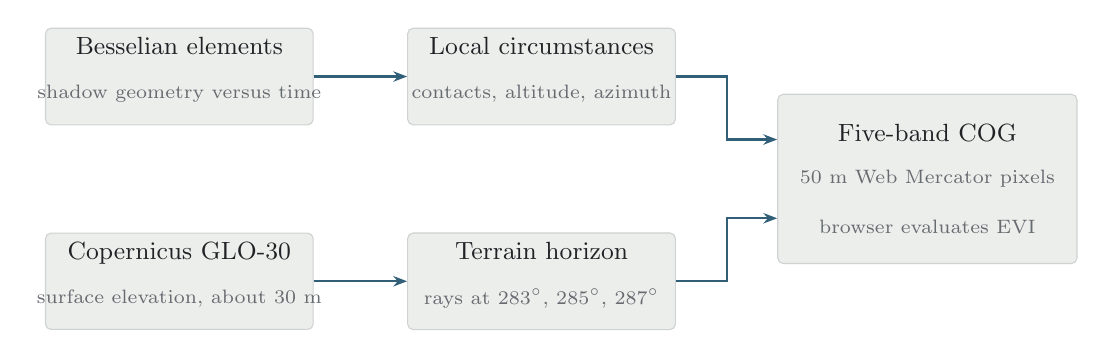
\begin{tikzpicture}[
  box/.style={draw=line,fill=panel,rounded corners=2pt,minimum width=3.4cm,
    minimum height=1.15cm,align=center,text=ink,font=\small},
  sub/.style={text=muted,font=\scriptsize},
  arrow/.style={draw=accent,line width=.8pt,-{Stealth[length=5pt]}}
]
\node[box] (elements) at (0,1.3) {Besselian elements\\[11pt]};
\node[sub] at (0,1.08) {shadow geometry versus time};
\node[box] (dem) at (0,-1.3) {Copernicus GLO-30\\[11pt]};
\node[sub] at (0,-1.52) {surface elevation, about 30 m};
\node[box] (circ) at (4.6,1.3) {Local circumstances\\[11pt]};
\node[sub] at (4.6,1.08) {contacts, altitude, azimuth};
\node[box] (horizon) at (4.6,-1.3) {Terrain horizon\\[11pt]};
\node[sub] at (4.6,-1.52) {rays at $283^\circ$, $285^\circ$, $287^\circ$};
\node[box,minimum width=3.8cm,minimum height=2.15cm] (cog) at (9.5,0)
  {Five-band COG\\[4pt]\textcolor{muted}{\scriptsize 50 m Web Mercator pixels}\\[7pt]
   \textcolor{muted}{\scriptsize browser evaluates EVI}};
\draw[arrow] (elements) -- (circ);
\draw[arrow] (dem) -- (horizon);
\draw[arrow] (circ.east) -- ++(.65,0) |- ([yshift=5mm]cog.west);
\draw[arrow] (horizon.east) -- ++(.65,0) |- ([yshift=-5mm]cog.west);
\end{tikzpicture}
\end{document}
